% =============================================================================
%  Fermiony Majorany — od drugiej kwantyzacji do nanodrutu
%
%  Części 1–4: wg plan.txt.  Część 5 („Realizacja fizyczna”): slajdy kolegi
%  z src/Majorany w nanodrucie warunki i eksperyment.pdf, wklejane jako strony.
%
%  Kompilacja:
%    make slajdy  -> slajdy.pdf               tylko części 1–4
%    make final   -> prezentacja_finalna.pdf  całość: części 1–4 + slajdy kolegi
%                    (prezentacja_finalna.tex ustawia \wersjafinalna na 1
%                     i wczytuje ten plik)
%
%  Wygląd (kremowe tło, granatowe slajdy działowe, EB Garamond + Inter,
%  kolory) jest skopiowany ze slajdów kolegi, żeby całość była jedną
%  prezentacją.  Wykresy: sim/wykresy.py -> fig/final/*.pdf.
%
%  Zasada: slajd pokazuje wzór / rysunek / hasło, resztę mówię.
% =============================================================================
\providecommand{\wersjafinalna}{0}
\documentclass[aspectratio=169,11pt]{beamer}
\usefonttheme{professionalfonts}

\usepackage{amsmath}
\usepackage{mathtools}
\usepackage{fontspec}
\usepackage{unicode-math}
% czcionki jak u kolegi: Inter (tekst), EB Garamond (tytuły, duże liczby)
\setsansfont{Inter}[Extension=.otf, UprightFont=*-Regular, ItalicFont=*-Italic,
  BoldFont=*-SemiBold, BoldItalicFont=*-SemiBoldItalic]
\setmainfont{EBGaramond}[Extension=.otf, UprightFont=*-Regular, ItalicFont=*-Italic,
  BoldFont=*-SemiBold, BoldItalicFont=*-SemiBoldItalic]
\newfontfamily\tytulowa{EBGaramond}[Extension=.otf, UprightFont=*-SemiBold,
  ItalicFont=*-SemiBoldItalic]
\setmathfont{Garamond-Math.otf}[Scale=1.1]
\setmonofont{JetBrains Mono}[Scale=MatchLowercase]
\usepackage{braket}
\usepackage[polish]{babel}
\usepackage{luavlna}
\singlechars{polish}{AaIiOoUuWwZz}
\usepackage{microtype}
\usepackage{newunicodechar}
% Inter nie ma tych znaków — bierzemy je z fontu matematycznego
\newunicodechar{⇒}{\ensuremath{\Rightarrow}}
\newunicodechar{⇓}{\ensuremath{\Downarrow}}
\usepackage{csquotes}
\DeclareQuoteAlias[guillemets*]{polish}{polish}
\usepackage{graphicx}
\usepackage{booktabs}
\usepackage{xcolor}
\usepackage{etoolbox}
\usepackage{siunitx}
\sisetup{per-mode=symbol, exponent-product=\cdot, output-decimal-marker={.}}
\usepackage{tikz}
\usetikzlibrary{arrows.meta, positioning, calc, decorations.pathmorphing, babel}

% --- prelegenci -----------------------------------------------------------------
\newcommand{\prelegentA}{Maciej}   % TODO: imię i nazwisko
\newcommand{\prelegentB}{}         % TODO: imię i nazwisko kolegi (część 5); puste = pomijamy
\newcommand{\dataWystapienia}{\today}  % TODO: data wystąpienia
\newcommand{\plikKolegi}{src/Majorany w nanodrucie warunki i eksperyment.pdf}

% --- kolory (próbkowane ze slajdów kolegi) ------------------------------------
\definecolor{tlo}{HTML}{F6F4EF}      % jasne tło
\definecolor{tloB}{HTML}{ECE7DC}     % beżowe tło (co drugi slajd)
\definecolor{mDark}{HTML}{172033}    % granat: tekst i slajdy działowe
\definecolor{mBlue}{HTML}{2D5BAA}    % elektron
\definecolor{mRed}{HTML}{A64B16}     % dziura, wyróżnienia (\alert)
\definecolor{mGreen}{HTML}{1F7A5A}
\definecolor{mPurple}{HTML}{6B3FA0}  % pół elektron, pół dziura
\definecolor{mGray}{HTML}{5A6170}
\definecolor{jasny}{HTML}{BFC8D9}    % tekst na granacie
\definecolor{linia}{HTML}{D0CABD}
\definecolor{kartabg}{HTML}{FBFBF8}
\definecolor{koral}{HTML}{D9534F}    % Majorany na końcach

% --- wygląd beamera -----------------------------------------------------------
\setbeamertemplate{navigation symbols}{}
\setbeamersize{text margin left=10.8mm, text margin right=10.8mm}
\setbeamercolor{normal text}{fg=mDark}
\setbeamercolor{structure}{fg=mDark}
\setbeamercolor{alerted text}{fg=mRed}
\setbeamerfont{frametitle}{family=\tytulowa, size=\fontsize{16.5}{19}}
\setbeamertemplate{frametitle}{%
  \nointerlineskip\vskip 8.6mm%
  {\usebeamerfont{frametitle}\color{mDark}\insertframetitle\par}%
  \vskip 1mm}
% tło: na przemian jasne i beżowe, jak u kolegi
\setbeamertemplate{background canvas}{%
  \ifodd\value{framenumber}\color{tloB}\else\color{tlo}\fi
  \vrule width\paperwidth height\paperheight}
% numer slajdu w prawym dolnym rogu (źródło — w lewym, jak u kolegi)
\setbeamertemplate{footline}{%
  \begin{tikzpicture}[remember picture, overlay]
    \node[anchor=base east, inner sep=0, text=mGray, font=\fontsize{6}{7}\selectfont]
      at ([xshift=-10.8mm, yshift=5.6mm]current page.south east) {\insertframenumber};
  \end{tikzpicture}%
  \rule{0pt}{9mm}}
\setbeamertemplate{itemize item}{\raisebox{0.22em}{\color{mRed}\rule{0.55em}{0.9pt}}}
\setbeamertemplate{itemize subitem}{\color{mGray}–}
\setlength{\leftmargini}{1.4em}
\hypersetup{pdftitle={Fermiony Majorany — od drugiej kwantyzacji do nanodrutu},
            pdfauthor={\prelegentA}}

% --- makra --------------------------------------------------------------------
% źródło rysunku/danych: lewy dolny róg
\newcommand{\zrodlo}[1]{%
  \begin{tikzpicture}[remember picture, overlay]
    \node[anchor=south west, inner sep=0, font=\fontsize{5.6}{6.8}\selectfont, text=mGray,
          text width=125mm, align=left]
      at ([xshift=10.8mm, yshift=4.3mm]current page.south west) {#1};
  \end{tikzpicture}}
% drobna uwaga na dole slajdu
\newcommand{\uwaga}[1]{\par\vfill{\fontsize{7.5}{9.2}\selectfont\color{mGray}#1\par}}
% duży tekst (EB Garamond) i podpis pod nim — jak „4 / stany przy μ” u kolegi
\newcommand{\duza}[1]{{\tytulowa\fontsize{22}{26}\selectfont #1}}
\newcommand{\podpis}[1]{{\fontsize{7.5}{9}\selectfont\color{mGray}#1}}
% karta z kolorowym paskiem: \karta[kolor]{szerokość}{treść}
\newcommand{\karta}[3][mRed]{%
  \begin{tikzpicture}[baseline=(k.base)]
    \node[fill=kartabg, draw=linia!70, line width=0.3pt, rounded corners=1.6pt,
          text width=#2, inner xsep=3mm, inner ysep=2.1mm, align=left,
          font=\small\bezdzielenia, text=mDark] (k) {#3};
    \fill[#1] ([xshift=0.15pt, yshift=-0.15pt]k.north west) rectangle ([xshift=0.9mm, yshift=0.15pt]k.south west);
  \end{tikzpicture}}
\newcommand{\bezdzielenia}{\hyphenpenalty=10000\exhyphenpenalty=10000\relax}
% rysunek z literatury na białej karcie (jak u kolegi): \obrazek{szerokość}{plik}
\newcommand{\obrazek}[2]{%
  \tikz\node[fill=white, draw=linia!70, line width=0.3pt, rounded corners=1.6pt,
             inner sep=1.6mm]{\includegraphics[width=#1]{#2}};}
\newcommand{\hc}{\mathrm{h.c.}}
\newcommand{\tak}{\tikz[baseline=-0.15ex]\draw[mGreen, line width=1.1pt, line cap=round,
  line join=round] (0,0.5ex) -- (0.38ex,0.08ex) -- (1.05ex,1.15ex);}
\newcommand{\nie}{\textcolor{mRed}{\ensuremath{\times}}}
\newcommand{\cz}[1]{\textcolor{mRed}{#1}}
\newcommand{\nb}[1]{\textcolor{mBlue}{#1}}
\newcommand{\LF}{[LF12]}

% granatowy slajd bez numeru
\newcommand{\ciemne}{\setbeamertemplate{background canvas}{\color{mDark}%
  \vrule width\paperwidth height\paperheight}}
% rysunek na całej stronie; współrzędne od lewego górnego rogu: (x, -y)
\newenvironment{naStronie}{%
  \begin{tikzpicture}[remember picture, overlay]
  \begin{scope}[shift={(current page.north west)}]}{%
  \end{scope}\end{tikzpicture}}

% mapa wystąpienia (pionowa, na slajdach działowych): #1 = bieżąca część
\newcommand{\etapy}{Cząstki i~antycząstki, Druga kwantyzacja, Majorany z~matematyki,
  Właściwości Majoran, Realizacja fizyczna}
\newcommand{\mapaPionowa}[1]{%
  \foreach \t [count=\i] in \etapy {
    \ifnum\i=#1\relax
      \node[anchor=base west, inner sep=0, font=\small, text=tlo]
        at (103mm,{-(26mm+\i*7.2mm)}) {\t};
      \node[anchor=base east, inner sep=0, font=\tytulowa\large, text=koral]
        at (99mm,{-(26mm+\i*7.2mm)}) {\i};
    \else
      \node[anchor=base west, inner sep=0, font=\small, text=jasny!45]
        at (103mm,{-(26mm+\i*7.2mm)}) {\t};
      \node[anchor=base east, inner sep=0, font=\tytulowa\large, text=jasny!35]
        at (99mm,{-(26mm+\i*7.2mm)}) {\i};
    \fi
  }
  \draw[jasny!30, line width=0.4pt] (95.5mm,{-(28mm)}) -- (95.5mm,{-(64mm)});}

% slajd otwierający część: \czesc{numer}{tytuł}{podtytuł}
\newcommand{\czesc}[3]{%
  \section{#2}%
  {\ciemne
  \begin{frame}[plain]
    \begin{naStronie}
      \node[anchor=base west, inner sep=0, font=\small, text=jasny]
        at (10.8mm,{-(24.5mm)}) {Część #1};
      \node[anchor=north west, inner sep=0, text=tlo, text width=80mm, align=left,
            font=\tytulowa\fontsize{26}{28}\selectfont\bezdzielenia] (t) at (10.8mm,{-(28.6mm)}) {#2};
      \node[anchor=north west, inner sep=0, text=jasny, text width=78mm, align=left,
            font=\fontsize{8.6}{11}\selectfont] at ([yshift=-4.5mm]t.south west) {#3};
      \mapaPionowa{#1}
    \end{naStronie}
  \end{frame}}}

% łańcuch Kitajewa (6 węzłów): #1 = 0 pary w węzłach, 1 pary sąsiednich połówek,
% 2 = jak 1 + nielokalny fermion z końców
\newcommand{\lancuch}[1]{%
  \begin{tikzpicture}[x=1cm, y=1cm]
    \foreach \i in {1,...,6} {
      \node[draw=linia, fill=kartabg, rounded corners=2pt, minimum width=1.02cm,
            minimum height=0.62cm] (w\i) at (1.32*\i, 0) {};
    }
    \ifnum#1=0\relax
      \foreach \i in {1,...,6}
        \draw[mBlue!70, dashed, thick] (1.32*\i, 0) ellipse (0.44 and 0.22);
      \foreach \i/\l in {1/1, 2/2, 3/3, 4/4, 5/5, 6/N}
        \node[below=1mm, font=\scriptsize] at (w\i.south) {$c_{\l}$};
      \foreach \i in {1,...,6} {
        \fill[mBlue] (1.32*\i-0.21, 0) circle (0.1);
        \fill[mBlue] (1.32*\i+0.21, 0) circle (0.1);
      }
    \else
      \foreach \i/\l in {1/1, 2/2, 3/3, 4/4, 5/{N-1}}
        \draw[mRed!80, dashed, thick] (1.32*\i+0.66, 0) ellipse (0.5 and 0.22)
          node[below=3.4mm, font=\scriptsize, text=mRed] {$\tilde c_{\l}$};
      \foreach \i in {1,...,6} {
        \fill[mBlue] (1.32*\i-0.21, 0) circle (0.1);
        \fill[mBlue] (1.32*\i+0.21, 0) circle (0.1);
      }
      \fill[koral!25] (1.32-0.21, 0) circle (0.2);
      \fill[koral] (1.32-0.21, 0) circle (0.11);
      \fill[koral!25] (6*1.32+0.21, 0) circle (0.2);
      \fill[koral] (6*1.32+0.21, 0) circle (0.11);
      \node[above=2.2mm, font=\scriptsize] at (1.32-0.21, 0) {$\gamma_{1,1}$};
      \node[above=2.2mm, font=\scriptsize] at (6*1.32+0.21, 0) {$\gamma_{N,2}$};
      \ifnum#1=2\relax
        \draw[koral, dashed, thick] (1.32-0.21, -0.72) .. controls (3.0,-1.45) and (6.6,-1.45)
          .. (6*1.32+0.21, -0.72)
          node[pos=0.5, below, font=\small, text=koral] {$\tilde c_M = \tfrac12\,(\gamma_{N,2} + i\gamma_{1,1})$};
      \fi
    \fi
  \end{tikzpicture}}

% =============================================================================
\title{Fermiony Majorany}
\subtitle{od drugiej kwantyzacji do nanodrutu}
\author{\prelegentA}
\date{\dataWystapienia}
\institute{Materiały i przyrządy półprzewodnikowe}

\begin{document}

% --- strona tytułowa -----------------------------------------------------------
{\ciemne
\begin{frame}[plain]
  \begin{naStronie}
    \node[anchor=north west, inner sep=0, text=tlo, align=left,
          font=\tytulowa\fontsize{30}{30}\selectfont] (t) at (10.8mm,{-(27.5mm)})
          {Fermiony\\Majorany};
    \node[anchor=north west, inner sep=0, text=jasny, font=\fontsize{9.5}{11}\selectfont]
      (p) at ([yshift=-4.6mm]t.south west) {od drugiej kwantyzacji do nanodrutu};
    \node[anchor=north west, inner sep=0, text=jasny, font=\fontsize{7}{8}\selectfont]
      at ([yshift=-5mm]p.south west)
      {\prelegentA\ifdefempty{\prelegentB}{}{\ \textperiodcentered\ \prelegentB}
       \ \textperiodcentered\ \dataWystapienia};
    \node[anchor=south west, inner sep=0, text=jasny!80, font=\fontsize{6}{7}\selectfont]
      at ([xshift=10.8mm, yshift=5.6mm]current page.south west)
      {Materiały i~przyrządy półprzewodnikowe};
    % łańcuch z Majoranami na końcach
    \begin{scope}[shift={(93mm,-46mm)}, x=1cm, y=1cm]
      \foreach \i in {0,...,4}
        \draw[jasny!35, rounded corners=2pt, fill=mDark!85!white] (1.12*\i-0.43,-0.27) rectangle (1.12*\i+0.43,0.27);
      \foreach \i in {0,...,3}
        \draw[jasny!60, dashed] (1.12*\i+0.56,0) ellipse (0.42 and 0.19);
      \foreach \i in {0,...,4} {
        \fill[tlo] (1.12*\i-0.18,0) circle (0.085);
        \fill[tlo] (1.12*\i+0.18,0) circle (0.085);
      }
      \foreach \x in {-0.18, 4.66} {
        \fill[koral!30] (\x,0) circle (0.2);
        \fill[koral] (\x,0) circle (0.1);
      }
      \node[text=koral, font=\small] at (-0.18,0.55) {$\gamma_1$};
      \node[text=koral, font=\small] at (4.66,0.55) {$\gamma_2$};
      \draw[koral!70, dashed, thick] (-0.18,-0.3) .. controls (0.8,-1.25) and (3.7,-1.25) .. (4.66,-0.3);
      \node[text=jasny, font=\scriptsize] at (2.24,-1.25) {jeden fermion na dwóch końcach};
    \end{scope}
  \end{naStronie}
\end{frame}}

% --- plan ---------------------------------------------------------------------
\begin{frame}{Plan}
  \centering
  \begin{tikzpicture}[
      etap/.style={fill=kartabg, draw=linia!70, line width=0.3pt, rounded corners=1.6pt,
                   text width=2.0cm, minimum height=1.55cm, align=left,
                   font=\footnotesize\bezdzielenia, inner xsep=2.3mm, text=mDark}]
    \foreach \t [count=\i] in \etapy {
      \node[etap] (n\i) at (2.78*\i, 0) {{\tytulowa\Large\color{mRed}\i}\\[0.5mm]\t};
      \fill[mRed] ([xshift=0.15pt, yshift=-0.15pt]n\i.north west) rectangle ([xshift=0.9mm, yshift=0.15pt]n\i.south west);
    }
    \foreach \i [evaluate=\i as \j using int(\i+1)] in {1,...,4}
      \draw[-{Stealth}, mGray, thick] (n\i) -- (n\j);
    \draw[mGray, line width=0.4pt] ([yshift=-3mm]n1.south west) -- ([yshift=-3mm]n4.south east);
    \node[below=4mm, font=\footnotesize, text=mGray] at ($(n2.south)!0.5!(n3.south)$) {\prelegentA};
    \draw[mGray, line width=0.4pt] ([yshift=-3mm]n5.south west) -- ([yshift=-3mm]n5.south east);
    \ifdefempty{\prelegentB}{}{%
      \node[below=4mm, font=\footnotesize, text=mGray] at (n5.south) {\prelegentB};}
  \end{tikzpicture}
\end{frame}

% =============================================================================
\czesc{1}{Cząstki i~antycząstki}{równanie Diraca, antymateria\\i~pomysł Majorany (1937)}
% =============================================================================

% plan: cząstki i antycząstki — równanie Diraca
\begin{frame}{Równanie Diraca (1928)}
  \centering
  \duza{$\bigl(i\hbar\,\gamma^\mu\partial_\mu - mc\bigr)\,\psi = 0$}\\[2mm]
  \podpis{postać hamiltonowska: \
    $i\hbar\,\partial_t\psi = \bigl(c\,\symbf{\alpha}\cdot\hat{\mathbf p} + \beta mc^2\bigr)\,\psi$}
  \\[8mm]
  \karta[mBlue]{3.75cm}{$\psi$ — spinor:\\ \textbf{4 składowe}\\[0.5mm]
    \footnotesize spin $\uparrow\downarrow$ \,×\, cząstka / antycząstka}\hfill
  \karta[mBlue]{3.75cm}{$\gamma^\mu$ — macierze $4\times4$\\[0.5mm]
    \footnotesize $\{\gamma^\mu,\gamma^\nu\} = 2\eta^{\mu\nu}$}\hfill
  \karta[mRed]{3.75cm}{$E = \pm\sqrt{p^2c^2 + m^2c^4}$\\[0.5mm]
    \footnotesize rozwiązania także\\ z~\alert{\mbox{$E < 0$}}}
  \uwaga{Spin $\tfrac12$ i~czynnik $g = 2$ elektronu wychodzą z~równania same.
    Algebra $\{\gamma^\mu,\gamma^\nu\} = 2\eta^{\mu\nu}$ wróci przy Majoranach: $\{\gamma_i,\gamma_j\} = 2\delta_{ij}$.}
  \zrodlo{P.\,A.\,M.~Dirac, Proc. R. Soc. Lond. A 117, 610 (1928)}
\end{frame}

% plan: cząstki i antycząstki — ujemne energie, morze Diraca
\begin{frame}{Ujemne energie: morze Diraca}
  \begin{columns}[c]
    \begin{column}{0.53\textwidth}
      \begin{itemize}\setlength{\itemsep}{3mm}
        \item stany z~$E<0$ są \alert{wszystkie zajęte} — „morze Diraca”
        \item dziura w~morzu = \alert{antycząstka}:\\ ta sama masa, przeciwny ładunek
        \item foton $\hbar\omega > 2mc^2$ tworzy parę $e^-e^+$
        \item pozyton $e^+$ — Anderson (1932)
      \end{itemize}
    \end{column}
    \begin{column}{0.43\textwidth}
      \centering
      \begin{tikzpicture}[scale=0.85]
        \fill[mBlue!12] (0,1) rectangle (3.4,2.8);
        \fill[mDark!22] (0,-1) rectangle (3.4,-2.8);
        \draw[-{Stealth}, mGray] (0,-3) -- (0,3.2) node[above, text=mDark] {$E$};
        \draw (-0.1,1) node[left] {$mc^2$} -- (0.1,1);
        \draw (-0.1,-1) node[left] {$-mc^2$} -- (0.1,-1);
        \node[font=\scriptsize, mBlue] at (1.3,2.45) {stany puste};
        \node[font=\scriptsize, mDark] at (1.3,-2.45) {stany obsadzone};
        \node[font=\scriptsize, mGray] at (1.1,0) {przerwa $2mc^2$};
        \draw[-{Stealth}, thick, mRed, decorate,
              decoration={snake, amplitude=1pt, segment length=5pt, post length=4pt}]
              (2.5,-1.45) -- (2.5,1.4);
        \fill[mBlue] (2.5,1.6) circle (3.5pt) node[right=3pt] {$e^-$};
        \draw[mRed, very thick, fill=tlo] (2.5,-1.65) circle (3.5pt) node[right=3pt] {$e^+$};
      \end{tikzpicture}
    \end{column}
  \end{columns}
  \zrodlo{C.\,D.~Anderson, Phys. Rev. 43, 491 (1933)}
\end{frame}

% plan: cząstki i antycząstki → pytanie Majorany
\begin{frame}{Czy cząstka może być własną antycząstką?}
  \centering
  \renewcommand{\arraystretch}{1.55}
  \begin{tabular}{llll}
    \toprule
    cząstka & antycząstka & & \\
    \midrule
    elektron $e^-$ & pozyton $e^+$ & różne & — \alert{ładunek} \\
    foton & foton & ta sama & — ale to \emph{bozon} \\
    neutrino $\nu$ & $\bar\nu$ ? & ? & — \alert{fermion}: wciąż otwarte \\
    \bottomrule
  \end{tabular}\\[9mm]
  \duza{fermion = swoja antycząstka?}
  \uwaga{Test dla neutrina: podwójny rozpad $\beta$ bez emisji neutrin — dotąd nie zaobserwowany.}
\end{frame}

% plan: cząstki i antycząstki → odpowiedź Majorany
\begin{frame}{Majorana (1937): rzeczywiste równanie Diraca}
  \begin{columns}[c]
    \begin{column}{0.5\textwidth}
      \centering
      macierze $\gamma^\mu$ wybrane \alert{czysto urojone}\\[2mm]
      \[ \bigl(\underbrace{i\hbar\,\gamma^\mu}_{\mathclap{\text{\footnotesize rzeczywiste}}}\partial_\mu - mc\bigr)\,\psi = 0 \]
      \vspace{1mm}
      $\psi$ jest rozwiązaniem ⇒ $\psi^*$ też\\[3mm]
      \duza{$\psi = \psi^*$}\\[1mm]
      \podpis{warunek Majorany}
    \end{column}
    \begin{column}{0.46\textwidth}
      \karta[mGreen]{5.3cm}{w~tej reprezentacji $\psi^*$ opisuje antycząstkę\\[0.5mm]
        ⇒ \textbf{cząstka = antycząstka}}\\[4mm]
      \karta[mRed]{5.3cm}{cena: \alert{brak ładunku}\\[0.5mm]
        \footnotesize pole $qA_\mu$ wnosi do równania $i$\\ ⇒ rzeczywiste tylko dla $q = 0$}
    \end{column}
  \end{columns}
  \zrodlo{E.~Majorana, Nuovo Cimento 14, 171 (1937)}
\end{frame}

% =============================================================================
\czesc{2}{Druga kwantyzacja}{jak opisać $10^{23}$ elektronów:\\operatory $c$ i~$c^\dagger$}
% =============================================================================

% plan: właściwości materiałów wynikają z kolektywnego oddziaływania elektronów
\begin{frame}{Materiał = wiele oddziałujących elektronów}
  \begin{columns}[c]
    \begin{column}{0.52\textwidth}
      \centering
      \begin{tikzpicture}
        \foreach \x in {0,...,6} \foreach \y in {0,...,3}
          \node[circle, fill=mDark!8, draw=mDark!30, inner sep=0pt, minimum size=4.5mm,
                font=\tiny, text=mGray] at (\x*0.95, \y*0.95) {$+$};
        \foreach \x/\y in {0.45/0.40, 1.35/1.40, 2.30/0.50, 3.10/2.35, 4.05/1.25,
                           4.90/2.65, 5.55/0.35, 0.50/2.30, 2.55/1.55, 3.70/0.20,
                           1.75/2.75, 5.20/1.60, 0.95/1.05, 4.40/0.55}
          \fill[mBlue] (\x,\y) circle (2.3pt);
        \draw[mBlue!55, decorate, decoration={snake, amplitude=0.7pt, segment length=3pt}]
          (1.35,1.40) -- (2.55,1.55)  (2.55,1.55) -- (3.10,2.35)
          (4.05,1.25) -- (5.20,1.60)  (0.45,0.40) -- (0.95,1.05)
          (2.30,0.50) -- (3.70,0.20)  (1.75,2.75) -- (3.10,2.35);
      \end{tikzpicture}
    \end{column}
    \begin{column}{0.44\textwidth}
      \duza{$\sim 10^{23}$}\\
      \podpis{elektronów w~\unit{\centi\metre\cubed}}\\[7mm]
      przewodnictwo · magnetyzm · nadprzewodnictwo\\[4mm]
      ⇒ zjawiska \alert{kolektywne}
    \end{column}
  \end{columns}
\end{frame}

% plan: podmienianie cząstek — dlaczego tylko faza? bozony i fermiony
\begin{frame}{Zamiana dwóch identycznych cząstek}
  \centering
  \begin{tikzpicture}
    \fill[mBlue] (0,0) circle (0.2) node[white, font=\scriptsize] {1};
    \fill[mBlue] (3.2,0) circle (0.2) node[white, font=\scriptsize] {2};
    \draw[-{Stealth}, thick, mRed] (0.25,0.22) to[bend left=35] (2.95,0.22);
    \draw[-{Stealth}, thick, mRed] (2.95,-0.22) to[bend left=35] (0.25,-0.22);
  \end{tikzpicture}
  \[ \psi(x_2, x_1) = e^{i\varphi}\,\psi(x_1, x_2) \]
  \begin{columns}[T]
    \begin{column}{0.45\textwidth}
      \centering
      nierozróżnialne ⇒ $|\psi|^2$ bez zmian\\
      ⇒ zmienia się tylko \alert{faza}
    \end{column}
    \begin{column}{0.45\textwidth}
      \centering
      dwie zamiany = brak zmiany\\
      ⇒ $e^{2i\varphi} = 1$ ⇒ \alert{$e^{i\varphi} = \pm1$}
    \end{column}
  \end{columns}
  \vspace{2mm}
  \karta[mBlue]{3.9cm}{$+1$: \textbf{bozony}\\[0.3mm] \footnotesize foton, fonon, $^4$He}\qquad
  \karta[mRed]{3.9cm}{$-1$: \textbf{fermiony}\\[0.3mm] \footnotesize elektron, proton, neutron}
  \uwaga{W~2D „dwie zamiany” to nie zawsze „brak zmiany” — wrócimy do tego przy statystyce nieabelowej.}
\end{frame}

% plan: skąd zakaz Pauliego akurat dla fermionów
\begin{frame}{Skąd zakaz Pauliego?}
  \begin{columns}[c]
    \begin{column}{0.48\textwidth}
      \centering
      dwa fermiony w~tym samym stanie:\\[2mm]
      $\psi(x, x) = -\psi(x, x)$\\[2mm]
      ⇓\\[2mm]
      \duza{$\psi(x, x) = 0$}\\[4mm]
      \alert{jeden fermion na stan}
    \end{column}
    \begin{column}{0.48\textwidth}
      \centering
      \begin{tikzpicture}[y=0.55cm]
        \foreach \y in {0,...,5} {
          \draw[thick, mGray!60] (0,\y) -- (1.8,\y);
          \draw[thick, mGray!60] (3,\y) -- (4.8,\y);
        }
        \foreach \x in {0.25,0.55,...,1.6} \fill[mGreen] (\x,0) ++(0,3.3pt) circle (3pt);
        \foreach \y in {0,...,3} \fill[mBlue] (3.9,\y) ++(0,3.3pt) circle (3pt);
        \draw[dashed, mRed, thick] (2.8,3.65) -- (5.0,3.65) node[right] {$E_F$};
        \node at (0.9,-1) {bozony};
        \node at (3.9,-1) {fermiony};
      \end{tikzpicture}
    \end{column}
  \end{columns}
\end{frame}

% plan: pierwsza kwantyzacja — wyznaczniki Slatera
\begin{frame}{Pierwsza kwantyzacja: wyznacznik Slatera}
  \[
    \Psi(x_1,\dots,x_N) = \frac{1}{\sqrt{N!}}
    \begin{vmatrix}
      \varphi_1(x_1) & \varphi_1(x_2) & \cdots & \varphi_1(x_N)\\
      \varphi_2(x_1) & \varphi_2(x_2) & \cdots & \varphi_2(x_N)\\
      \vdots & \vdots & \ddots & \vdots\\
      \varphi_N(x_1) & \varphi_N(x_2) & \cdots & \varphi_N(x_N)
    \end{vmatrix}
  \]
  \vspace{4mm}
  \begin{columns}[T]
    \begin{column}{0.42\textwidth}
      \centering
      zamiana kolumn → znak $-$\\[1mm]
      \tak\ antysymetria
    \end{column}
    \begin{column}{0.42\textwidth}
      \centering
      dwa takie same wiersze → $0$\\[1mm]
      \tak\ zakaz Pauliego
    \end{column}
  \end{columns}
\end{frame}

% plan: problemy — kosztowne obliczenia, z góry ustalone N; potrzebna rewolucja
\begin{frame}{Problemy}
  \begin{columns}[T]
    \begin{column}{0.42\textwidth}
      \centering
      \duza{$N!$}\\
      \podpis{składników}\\[3mm]
      \renewcommand{\arraystretch}{1.15}
      \begin{tabular}{rr}
        $N$ & $N!$\\
        \midrule
        3  & 6\\
        10 & \num{3628800}\\
        20 & \num{2.4e18}\\
      \end{tabular}
    \end{column}
    \begin{column}{0.42\textwidth}
      \centering
      \duza{$N$}\\
      \podpis{ustalone z~góry}\\[4mm]
      a~co, gdy cząstki\\
      \alert{powstają i~znikają}?
    \end{column}
  \end{columns}
  \vfill
  \centering
  \karta[mRed]{12.6cm}{zamiast „\emph{która} cząstka \emph{gdzie}?” \quad → \quad
    „\alert{\emph{ile} cząstek w~\emph{którym} stanie?}”}
\end{frame}

% plan: przejście na drugą kwantyzację
\begin{frame}{Druga kwantyzacja: liczby obsadzeń}
  \begin{columns}[c]
    \begin{column}{0.4\textwidth}
      \centering
      \begin{tikzpicture}[y=0.7cm]
        \foreach \i/\n in {1/1, 2/0, 3/1, 4/1, 5/0} {
          \draw[thick, mGray!60] (0,\i) -- (1.8,\i);
          \node[left] at (0,\i) {$\varphi_\i$};
          \node[right, font=\small] at (2.0,\i) {$n_\i = \n$};
          \ifnum\n=1 \fill[mBlue] (0.9,\i) ++(0,4pt) circle (3.5pt); \fi
        }
        \node at (1.3,0) {$\ket{1,0,1,1,0}$};
      \end{tikzpicture}
    \end{column}
    \begin{column}{0.55\textwidth}
      \centering
      \textcolor{mGray}{$\Psi(x_1,\dots,x_N)$}\\[2mm]
      ⇓\\[2mm]
      \duza{$\ket{n_1, n_2, n_3, \dots}$}\\[7mm]
      fermiony: \alert{$n_i \in \{0, 1\}$}\\[3mm]
      $N = \sum_i n_i$ — \alert{nie musi być stałe}
    \end{column}
  \end{columns}
\end{frame}

% plan: pojedynczy fermion — zero lub jeden — kubit; 2-wymiarowa przestrzeń;
%       ortonormalność i zupełność
\begin{frame}{Jeden stan fermionowy}
  \begin{columns}[c]
    \begin{column}{0.42\textwidth}
      \centering
      \begin{tikzpicture}
        \draw[thick, mGray!60] (0,0) -- (1.5,0);
        \node[below=3pt] at (0.75,0) {$\ket{0}$ pusty};
        \draw[thick, mGray!60] (2.8,0) -- (4.3,0);
        \fill[mBlue] (3.55,0) ++(0,4pt) circle (3.5pt);
        \node[below=3pt] at (3.55,0) {$\ket{1}$ zajęty};
      \end{tikzpicture}\\[9mm]
      \duza{$\dim\mathcal{H} = 2$}\\
      \podpis{lokalna przestrzeń Hilberta — jak \alert{kubit}}
    \end{column}
    \begin{column}{0.54\textwidth}
      ortonormalność
      \[ \braket{0|0} = \braket{1|1} = 1, \qquad \braket{0|1} = 0 \]
      zupełność
      \[ \ket0\bra0 + \ket1\bra1 = \mathbb{1} \]
      \[
        \ket0 = \begin{pmatrix}1\\0\end{pmatrix}, \qquad
        \ket1 = \begin{pmatrix}0\\1\end{pmatrix}
      \]
    \end{column}
  \end{columns}
  \uwaga{„0” i~„1” to na razie tylko \emph{nazwy} stanów.}
\end{frame}

% plan: operatory kreacji i anihilacji, zasady działania, postać ketbra
\begin{frame}{Operatory kreacji i~anihilacji}
  \begin{columns}[c]
    \begin{column}{0.42\textwidth}
      \centering
      \begin{tikzpicture}[
          st/.style={draw=linia, fill=kartabg, rounded corners=3pt, minimum width=1.4cm, minimum height=0.8cm}]
        \node[st] (z) at (0,0) {$\ket0$};
        \node[st] (j) at (0,2.6) {$\ket1$};
        \draw[-{Stealth}, very thick, mBlue] ([xshift=-3mm]z.north) to[bend left=35]
          node[left] {$c^\dagger$} ([xshift=-3mm]j.south);
        \draw[-{Stealth}, very thick, mRed] ([xshift=3mm]j.south) to[bend left=35]
          node[right] {$c$} ([xshift=3mm]z.north);
        \node[mGray] (o1) at (2.3,2.6) {$0$};
        \draw[-{Stealth}, mGray, dashed] (j.east) -- node[above, font=\scriptsize] {$c^\dagger$} (o1);
        \node[mGray] (o0) at (2.3,0) {$0$};
        \draw[-{Stealth}, mGray, dashed] (z.east) -- node[below, font=\scriptsize] {$c$} (o0);
      \end{tikzpicture}
    \end{column}
    \begin{column}{0.54\textwidth}
      \[ c^\dagger = \ket1\bra0, \qquad c = \ket0\bra1 \]
      \begin{align*}
        c^\dagger\ket0 &= \ket1, & c^\dagger\ket1 &= 0,\\
        c\ket1 &= \ket0, & c\ket0 &= 0.
      \end{align*}
      \[
        c^\dagger = \begin{pmatrix}0&0\\1&0\end{pmatrix}, \qquad
        c = \begin{pmatrix}0&1\\0&0\end{pmatrix}
      \]
    \end{column}
  \end{columns}
\end{frame}

% plan: (dlaczego) operatory są zupełne — ich span to cała przestrzeń operatorów
\begin{frame}{Dlaczego $c$ i~$c^\dagger$ wystarczą?}
  \centering
  każdy operator na tym stanie to macierz $2\times2$\\[5mm]
  \begin{columns}[c]
    \begin{column}{0.35\textwidth}
      \centering
      \[
        \hat O = \begin{pmatrix} O_{00} & O_{01}\\ O_{10} & O_{11}\end{pmatrix}
      \]
    \end{column}
    \begin{column}{0.5\textwidth}
      \centering
      \renewcommand{\arraystretch}{1.8}
      \begin{tabular}{c|c}
        $\ket0\bra0 = \cz{c\,c^\dagger}$ & $\ket0\bra1 = \cz{c}$ \\
        \hline
        $\ket1\bra0 = \cz{c^\dagger}$ & $\ket1\bra1 = \cz{c^\dagger c}$
      \end{tabular}
    \end{column}
  \end{columns}
  \vspace{6mm}
  \[
    \hat O = O_{00}\,c\,c^\dagger + O_{01}\,c + O_{10}\,c^\dagger + O_{11}\,c^\dagger c
  \]
  \uwaga{Cztery iloczyny $c$, $c^\dagger$ rozpinają całą przestrzeń operatorów $2\times2$.}
\end{frame}

% plan: operatory nie są hermitowskie → w hamiltonianie tylko parami
\begin{frame}{Hamiltonian: operatory parami}
  \centering
  $c^\dagger \neq c$ \quad ⇒ \quad nie są hermitowskie — \alert{nie są obserwablami}\\[3mm]
  $H = H^\dagger$ \quad ⇒ \quad $c$ i~$c^\dagger$ występują \alert{parami}\\[8mm]
  \renewcommand{\arraystretch}{1.6}
  \begin{tabular}{cll}
    \nie & $c$, \ $c^\dagger$ & \\
    \tak & $\varepsilon\,c^\dagger c$ & energia stanu \\
    \tak & $c_i^\dagger c_j + c_j^\dagger c_i$ & przeskok $i \leftrightarrow j$ \\
    \tak & $c_i c_j + c_j^\dagger c_i^\dagger$ & parowanie \textcolor{mGray}{(przyda się!)} \\
  \end{tabular}
\end{frame}

% plan: c†c jako operator liczby obsadzeń, wartości własne {0,1}, hermitowskość;
%       operator liczby obsadzeń jako jedyne, co można wstawić do hamiltonianu
\begin{frame}{Operator liczby obsadzeń $\hat n = c^\dagger c$}
  \begin{columns}[c]
    \begin{column}{0.5\textwidth}
      \begin{align*}
        \hat n\ket0 &= c^\dagger c\ket0 = \cz{0}\cdot\ket0\\
        \hat n\ket1 &= c^\dagger c\ket1 = \cz{1}\cdot\ket1
      \end{align*}
      \[ \hat n^\dagger = (c^\dagger c)^\dagger = c^\dagger c = \hat n \]
      \centering
      hermitowski ⇒ \alert{obserwabla}
    \end{column}
    \begin{column}{0.46\textwidth}
      \centering
      wartości własne $\{0, 1\}$\\[1mm]
      ⇓\\[1mm]
      „0” i~„1” to \alert{liczba cząstek} w~stanie\\[6mm]
      \karta[mRed]{5cm}{\centering jeden stan: \ $H = \varepsilon\,\hat n$\\[0.3mm]
        \footnotesize nic innego do $H$ nie wstawimy}
    \end{column}
  \end{columns}
  \uwaga{$\hat N = \sum_i \hat n_i$ liczy wszystkie cząstki.
    Człony z~nieparzystą liczbą $c$ zmieniają parzystość liczby fermionów — fizyczny $H$ ich nie zawiera.}
\end{frame}

% plan: wszystkie relacje komutacji i antykomutacji
\begin{frame}{Relacje antykomutacji}
  \begin{columns}[T]
    \begin{column}{0.52\textwidth}
      \karta[mRed]{5.6cm}{\textbf{fermiony:} \ $\{A,B\} = AB + BA$
        \vspace{-2mm}
        \begin{align*}
          \{c_i, c_j^\dagger\} &= \delta_{ij}\\
          \{c_i, c_j\} &= \{c_i^\dagger, c_j^\dagger\} = 0
        \end{align*}}\\[4mm]
      $(c_i^\dagger)^2 = 0$ \hfill → \alert{zakaz Pauliego}\\[2mm]
      $c_i^\dagger c_j^\dagger = -c_j^\dagger c_i^\dagger$ \hfill → \alert{antysymetria}
    \end{column}
    \begin{column}{0.42\textwidth}
      \karta[mBlue]{4.4cm}{\textbf{bozony:} \ $[A,B] = AB - BA$
        \vspace{-2mm}
        \[ [a_i, a_j^\dagger] = \delta_{ij}, \quad [a_i, a_j] = 0 \]}\\[4mm]
      \centering
      $\hat n$ liczy cząstki:
      \begin{align*}
        [\hat n_i, c_j^\dagger] &= +\delta_{ij}\,c_j^\dagger\\
        [\hat n_i, c_j] &= -\delta_{ij}\,c_j
      \end{align*}
    \end{column}
  \end{columns}
\end{frame}

% plan: zalety formalizmu
\begin{frame}{Co zyskujemy}
  \centering
  cały układ wielu ciał w~jednej linii:
  \[
    H = \underbrace{\sum_{ij} t_{ij}\, c_i^\dagger c_j}_{\mathclap{\text{\small ruch}}}
      \;+\; \underbrace{\frac12 \sum_{ijkl} V_{ijkl}\, c_i^\dagger c_j^\dagger c_l c_k}_{\mathclap{\text{\small oddziaływanie}}}
  \]
  \vspace{6mm}
  \karta[mBlue]{3.75cm}{\centering \alert{statystyka}\\ wbudowana w~algebrę}\hfill
  \karta[mBlue]{3.75cm}{\centering $N$ \alert{nie} jest\\ ustalone}\hfill
  \karta[mBlue]{3.75cm}{\centering rachunki = \alert{(anty)komutatory}\\ zamiast wyznaczników}
\end{frame}

% =============================================================================
\czesc{3}{Majorany z~matematyki}{połówki fermionu, nadprzewodnik\\i~łańcuch Kitajewa}
% =============================================================================

% plan: w ciele stałym c, c† dotyczą elektronów i dziur
\begin{frame}{W~ciele stałym: elektrony i~dziury}
  \begin{columns}[c]
    \begin{column}{0.44\textwidth}
      \centering
      \begin{tikzpicture}
        \fill[mDark!20] (0,0) rectangle (3.4,1.6);
        \fill[mBlue!8] (0,1.6) rectangle (3.4,3.2);
        \draw[-{Stealth}, mGray] (-0.3,0) -- (-0.3,3.4) node[above, text=mDark] {$E$};
        \draw[dashed, mRed, thick] (-0.1,1.6) -- (3.5,1.6) node[right] {$E_F$};
        \node[font=\scriptsize] at (1.7,0.25) {stany obsadzone};
        \node[font=\scriptsize] at (1.7,2.95) {stany puste};
        \fill[mBlue] (1.0,2.3) circle (4pt) node[right=4pt] {$e^-$};
        \draw[mRed, very thick, fill=tlo] (2.3,0.9) circle (4pt) node[right=4pt] {$h^+$};
      \end{tikzpicture}
    \end{column}
    \begin{column}{0.52\textwidth}
      $c^\dagger$ — dodaje elektron \hfill \nb{$-e$}\\[4mm]
      $c$ — zabiera elektron = tworzy \alert{dziurę} \hfill \cz{$+e$}\\[10mm]
      \centering
      dziura = „antycząstka” elektronu\\
      \podpis{(jak pozyton w~morzu Diraca)}
    \end{column}
  \end{columns}
\end{frame}

% plan: idea — pół zwykłego fermionu; rozdzielenie operatorów kreacji i anihilacji
\begin{frame}{Pomysł: fermion z~dwóch „połówek”}
  \begin{columns}[c]
    \begin{column}{0.42\textwidth}
      \centering
      \begin{tikzpicture}
        \fill[mBlue] (0,0.9) arc (90:270:0.9) -- cycle;
        \fill[mRed] (0,-0.9) arc (-90:90:0.9) -- cycle;
        \node at (0,-1.3) {$c$};
        \draw[-{Stealth}, thick, mGray] (1.2,0) -- (2.0,0);
        \fill[mBlue] (3.1,0.9) arc (90:270:0.9) -- cycle;
        \fill[mRed] (3.7,-0.9) arc (-90:90:0.9) -- cycle;
        \node[white] at (2.72,0) {$\gamma_1$};
        \node[white] at (4.08,0) {$\gamma_2$};
      \end{tikzpicture}
    \end{column}
    \begin{column}{0.54\textwidth}
      \centering
      \duza{$c = \tfrac12\,(\gamma_1 + i\gamma_2)$}\\
      \podpis{jak \ $z = x + iy$}\\[6mm]
      \[ \gamma_1 = c + c^\dagger, \qquad \gamma_2 = i\,(c^\dagger - c) \]
      „część rzeczywista” i~„urojona” fermionu
    \end{column}
  \end{columns}
\end{frame}

% plan: superpozycja fermionu i antycząstki = elektronu i dziury; hermitowskie;
%       własna antycząstka → nie są zwykłymi fermionami
\begin{frame}{Majorana = elektron + dziura}
  \centering
  \begingroup\LARGE
  \[
    \gamma_1 = \underset{\text{\normalsize\color{mBlue}elektron}}{\textcolor{mBlue}{c^\dagger}}
             \;+\; \underset{\text{\normalsize\color{mRed}dziura}}{\textcolor{mRed}{c}}
  \]
  \endgroup
  \vspace{1mm}
  cząstka i~antycząstka \alert{w~równych proporcjach}\\[8mm]
  \duza{$\gamma^\dagger = \gamma$} \quad
  ⇒ \quad \alert{cząstka = własna antycząstka}\\[6mm]
  \podpis{w~układzie fermionów coś niezwykłego: $\gamma$ nie jest zwykłym fermionem}
\end{frame}

% plan: gdzie szukać? półprzewodniki — nie można mieszać e i h (ładunek)
\begin{frame}{Gdzie szukać? Półprzewodnik — nie}
  \centering
  \vfill
  \begin{tikzpicture}
    \node (s) {\LARGE $u\,\ket{e^-} + v\,\ket{h^+}$};
    \node[right=5mm of s, text=mRed, font=\Huge] {$\times$};
  \end{tikzpicture}\\[6mm]
  ładunek \nb{$-e$} \quad i \quad ładunek \cz{$+e$}\\[2mm]
  \alert{zasada zachowania ładunku} zabrania takiej superpozycji\\[10mm]
  potrzebny układ, w~którym ładunek elektronu może „zniknąć”
  \vfill
\end{frame}

% plan: wstęp do nadprzewodników
\begin{frame}{Nadprzewodnik}
  \begin{columns}[c]
    \begin{column}{0.48\textwidth}
      \centering
      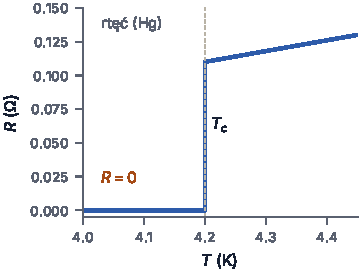
\includegraphics[width=\linewidth]{fig/final/opor_T.pdf}
    \end{column}
    \begin{column}{0.48\textwidth}
      \karta[mBlue]{5.4cm}{poniżej $T_c$ opór \alert{dokładnie zero}\\[0.3mm]
        \footnotesize Kamerlingh Onnes 1911, rtęć}\\[3mm]
      \karta[mBlue]{5.4cm}{pole magnetyczne \alert{wypchnięte}\\[0.3mm]
        \footnotesize efekt Meissnera 1933}\\[3mm]
      \karta[mBlue]{5.4cm}{Al: $T_c = \qty{1.2}{K}$, \ Pb: \qty{7.2}{K}, \ Nb: \qty{9.3}{K}}
    \end{column}
  \end{columns}
  \zrodlo{Wykres schematyczny; H.~Kamerlingh Onnes, Commun. Phys. Lab. Leiden 120b (1911);
    W.~Meissner, R.~Ochsenfeld, Naturwissenschaften 21, 787 (1933)}
\end{frame}

% plan: pary Coopera — skąd przyciąganie (defekt sieci, jony wolniejsze od elektronu)
\begin{frame}{Para Coopera: skąd przyciąganie?}
  \centering
  \begin{tikzpicture}[x=1cm, y=1cm]
    \def\xe{8.3}
    \fill[mRed!13] (5.6,0) ellipse (2.1 and 0.42);
    \foreach \i in {0,...,11} {
      \pgfmathsetmacro\x{0.8*\i}
      \pgfmathsetmacro\d{(\x<\xe)*0.3*exp(-((\xe-\x)-2.6)^2/3.0)}
      \node[circle, fill=mDark!8, draw=mDark!30, inner sep=0pt, minimum size=4mm,
            font=\tiny, text=mGray] at (\x, 0.8-\d) {$+$};
      \node[circle, fill=mDark!8, draw=mDark!30, inner sep=0pt, minimum size=4mm,
            font=\tiny, text=mGray] at (\x, -0.8+\d) {$+$};
    }
    \fill[mBlue] (\xe,0) circle (3.2pt);
    \draw[-{Stealth}, thick, mBlue] (\xe+0.15,0) -- (\xe+1.0,0) node[right, font=\scriptsize] {$e^-$, \ $v_F \sim \qty{e6}{m/s}$};
    \node[font=\scriptsize, text=mRed] at (5.5,-1.45) {ślad: nadmiar ładunku dodatniego};
    \fill[mBlue] (1.0,0) circle (3.2pt) node[below=2pt, font=\scriptsize] {drugi $e^-$};
    \draw[-{Stealth}, thick, mBlue!70, dashed] (1.2,0) -- (3.4,0);
  \end{tikzpicture}\\[7mm]
  \karta[mBlue]{2.65cm}{\footnotesize\textbf{1.} elektron przyciąga jony — sieć się odkształca}\hfill
  \karta[mBlue]{2.65cm}{\footnotesize\textbf{2.} jony są ciężkie: reagują \alert{wolno}, elektron jest już daleko}\hfill
  \karta[mBlue]{2.65cm}{\footnotesize\textbf{3.} zostaje „ślad” ładunku dodatniego}\hfill
  \karta[mRed]{2.65cm}{\footnotesize\textbf{4.} ślad przyciąga drugi elektron → \alert{para}}
  \uwaga{Skale: $\hbar\omega_D \sim 10$–$\qty{40}{meV}$ (drgania sieci) \ $\ll$ \ $E_F \sim \qty{10}{eV}$ (elektrony).}
\end{frame}

% plan: przeciwne pędy i spiny — wzór
\begin{frame}{Para Coopera: przeciwne pędy i~spiny}
  \begin{columns}[c]
    \begin{column}{0.53\textwidth}
      \centering
      \[ \ket{\text{para}} = \sum_{\mathbf k} g_{\mathbf k}\;
         c^\dagger_{\mathbf k\uparrow}\,c^\dagger_{-\mathbf k\downarrow}\,\ket{F} \]
      \podpis{$\ket{F}$ — zapełnione morze Fermiego}\\[5mm]
      \karta[mBlue]{5.6cm}{pęd: \ $\hbar\mathbf k + \hbar(-\mathbf k) = 0$}\\[2.5mm]
      \karta[mBlue]{5.6cm}{spin: \ $\uparrow\downarrow$ — singlet, $S = 0$}
    \end{column}
    \begin{column}{0.43\textwidth}
      \centering
      \begin{tikzpicture}[scale=0.82]
        \fill[mBlue!25, even odd rule] (0,0) circle (1.25) (0,0) circle (1.0);
        \draw[mBlue] (0,0) circle (1.25) (0,0) circle (1.0);
        \node[font=\scriptsize, align=center] at (0,-1.75) {$\mathbf K = 0$\\cała warstwa};
        \begin{scope}[xshift=3.2cm]
          \begin{scope}[even odd rule]
            \clip (-0.25,0) circle (1.25) (-0.25,0) circle (1.0);
            \fill[mPurple!40, even odd rule] (0.25,0) circle (1.25) (0.25,0) circle (1.0);
          \end{scope}
          \draw[mBlue] (-0.25,0) circle (1.25) (-0.25,0) circle (1.0);
          \draw[mRed] (0.25,0) circle (1.25) (0.25,0) circle (1.0);
          \node[font=\scriptsize, align=center] at (0,-1.75) {$\mathbf K \neq 0$\\tylko część};
        \end{scope}
      \end{tikzpicture}\\[1mm]
      \podpis{przyciąganie działa tylko w~cienkiej warstwie przy $E_F$;\\
        para o~pędzie $\mathbf K = 0$ ma \alert{najwięcej} stanów do dyspozycji}
    \end{column}
  \end{columns}
  \uwaga{Energia wiązania $\approx 2\hbar\omega_D\,e^{-2/N(0)V}$ — wystarcza dowolnie słabe przyciąganie.}
  \zrodlo{L.\,N.~Cooper, Phys. Rev. 104, 1189 (1956)}
\end{frame}

% plan: przeciwny pęd ≠ ruch w przeciwne strony; krążą wokół siebie; pary ogromne
\begin{frame}{Para jest ogromna}
  \begin{columns}[c]
    \begin{column}{0.42\textwidth}
      \centering
      \begin{tikzpicture}
        \foreach \x/\y in {-0.9/0.5, 0.8/0.7, 0.3/-0.8, -0.6/-0.6, 1.0/-0.2}
          \draw[mPurple!30] (\x,\y) circle (1.15);
        \draw[mPurple, thick, dashed] (0,0) circle (1.15);
        \fill[mBlue] (1.15,0) circle (3pt);
        \fill[mBlue] (-1.15,0) circle (3pt);
        \draw[-{Stealth}, mBlue, thick] (1.15,0.15) arc (0:28:1.15);
        \draw[-{Stealth}, mBlue, thick] (-1.15,-0.15) arc (180:208:1.15);
        \draw[{Stealth}-{Stealth}, mGray] (-1.15,-1.55) -- node[below, font=\scriptsize] {$\xi_0$} (1.15,-1.55);
      \end{tikzpicture}
    \end{column}
    \begin{column}{0.54\textwidth}
      \duza{$\xi_0 \approx \qty{1.6}{\micro\metre}$}\\
      \podpis{rozmiar pary w~Al $\approx 4000$ stałych sieci}\\[4mm]
      \begin{itemize}\setlength{\itemsep}{2mm}
        \item przeciwne pędy $\neq$ ruch w~przeciwne strony: para to \alert{superpozycja} wszystkich $(\mathbf k, -\mathbf k)$
        \item obraz: elektrony „krążą wokół siebie”
        \item w~objętości jednej pary — \alert{miliony} innych par
      \end{itemize}
    \end{column}
  \end{columns}
  \uwaga{$\xi_0 = \hbar v_F/\pi\Delta$: \ Al \qty{1600}{nm}, \ Sn \qty{230}{nm}, \ Pb \qty{83}{nm}, \ Nb \qty{38}{nm}.}
  \zrodlo{Ch.~Kittel, \emph{Introduction to Solid State Physics}, rozdz.~10}
\end{frame}

% plan: kondensat par Coopera — może przyjąć albo oddać parę 2e
\begin{frame}{Kondensat par Coopera}
  \begin{columns}[c]
    \begin{column}{0.46\textwidth}
      \centering
      \begin{tikzpicture}
        \draw[rounded corners=8pt, fill=mPurple!8, draw=mPurple!40] (0,0) rectangle (4,2.2);
        \foreach \x/\y in {0.7/0.6, 2.0/0.6, 3.3/0.6, 1.1/1.6, 2.4/1.6, 3.4/1.6} {
          \draw[mPurple!60] (\x,\y) ellipse (0.32 and 0.18);
          \fill[mBlue] (\x-0.13,\y) circle (1.8pt);
          \fill[mBlue] (\x+0.13,\y) circle (1.8pt);
        }
        \node[font=\scriptsize, text=mPurple] at (2,-0.3) {jeden stan: $\Psi = |\Psi|\,e^{i\varphi}$};
        \draw[mPurple!60] (5.35,1.1) ellipse (0.32 and 0.18);
        \fill[mBlue] (5.22,1.1) circle (1.8pt);
        \fill[mBlue] (5.48,1.1) circle (1.8pt);
        \draw[{Stealth}-{Stealth}, thick, mRed] (4.15,1.1) --
          node[below, font=\scriptsize] {$2e$} (4.95,1.1);
      \end{tikzpicture}
    \end{column}
    \begin{column}{0.5\textwidth}
      \begin{itemize}\setlength{\itemsep}{2.5mm}
        \item para: spin $0$ → zachowuje się jak \alert{bozon}
        \item wszystkie pary w~\alert{jednym} stanie — kondensat
        \item kondensat może \alert{przyjąć lub oddać} parę ($2e$) bez kosztu energii
      \end{itemize}
      \vspace{3mm}
      \karta[mRed]{5.5cm}{liczba elektronów ustalona tylko co do $2$\\[0.3mm]
        \footnotesize zachowana jest \alert{parzystość} — przyda się}
    \end{column}
  \end{columns}
  \zrodlo{J.~Bardeen, L.\,N.~Cooper, J.\,R.~Schrieffer, Phys. Rev. 108, 1175 (1957)}
\end{frame}

% plan: przerwa energetyczna jako fakt doświadczalny; od dowolnie małego napięcia vs przerwa
\begin{frame}{Przerwa energetyczna: fakt doświadczalny}
  \begin{columns}[c]
    \begin{column}{0.47\textwidth}
      \centering
      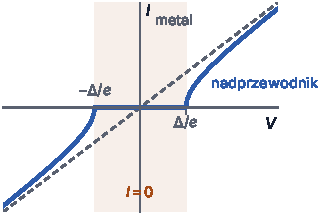
\includegraphics[width=\linewidth]{fig/final/przerwa_IV.pdf}\\
      \podpis{złącze tunelowe: metal | izolator | ?, \ $T = 0$}
    \end{column}
    \begin{column}{0.49\textwidth}
      \karta[mGray]{5.4cm}{\textbf{metal:} prąd płynie od \alert{dowolnie małego} napięcia}\\[3mm]
      \karta[mBlue]{5.4cm}{\textbf{nadprzewodnik:} $I = 0$ aż do $eV = \Delta$}\\[3mm]
      \karta[mRed]{5.4cm}{nawet w~$T = 0$ najtańsze wzbudzenie kosztuje \alert{skończoną} energię}
    \end{column}
  \end{columns}
  \zrodlo{I.~Giaever, Phys. Rev. Lett. 5, 147 (1960); wykres: $I \propto \sqrt{(eV)^2 - \Delta^2}$ dla $|eV| > \Delta$}
\end{frame}

% plan: każdy nadprzewodnik ma własną przerwę; rzędu meV ≪ E_F; rozerwanie pary
\begin{frame}{Przerwa energetyczna: skala}
  \begin{columns}[c]
    \begin{column}{0.52\textwidth}
      \centering
      \renewcommand{\arraystretch}{1.3}
      \setlength{\tabcolsep}{3.5pt}
      \small
      \begin{tabular}{lrrrr}
        \toprule
           & $T_c$ & $\Delta$ & $E_F$ & $\Delta/E_F$ \\
        \midrule
        Al & \qty{1.2}{K} & \qty{0.17}{meV} & \qty{11.7}{eV} & \num{1.5e-5} \\
        Sn & \qty{3.7}{K} & \qty{0.58}{meV} & \qty{10.2}{eV} & \num{5.7e-5} \\
        Pb & \qty{7.2}{K} & \qty{1.37}{meV} & \qty{9.5}{eV}  & \num{1.4e-4} \\
        Nb & \qty{9.3}{K} & \qty{1.5}{meV}  & \qty{5.3}{eV}  & \num{2.9e-4} \\
        \bottomrule
      \end{tabular}\\[3mm]
      \podpis{każdy nadprzewodnik ma \alert{własną} przerwę; \ BCS: $2\Delta \approx 3.5\,k_BT_c$}
    \end{column}
    \begin{column}{0.44\textwidth}
      \centering
      \duza{$\Delta \ll E_F$}\\
      \podpis{przerwa dotyczy tylko cienkiej warstwy stanów przy $E_F$}\\[6mm]
      \karta[mRed]{5cm}{wzbudzić nadprzewodnik\\ = \alert{rozerwać parę}: \ $2\Delta$\\[0.3mm]
        \footnotesize dwie kwazicząstki, każda $\ge \Delta$}
    \end{column}
  \end{columns}
  \zrodlo{Ch.~Kittel, \emph{Introduction to Solid State Physics}, tab.~10.3 ($\Delta = \tfrac12\cdot$przerwa);
    $E_F$ z~modelu elektronów swobodnych: N.\,W.~Ashcroft, N.\,D.~Mermin, \emph{Solid State Physics}, tab.~2.1}
\end{frame}

% plan: odbicie Andreeva
\begin{frame}{Odbicie Andriejewa}
  \centering
  \begin{tikzpicture}[x=1cm, y=1cm]
    \fill[kartabg] (0,0) rectangle (5.2,2.9);
    \fill[mPurple!9] (5.2,0) rectangle (9.6,2.9);
    \draw[linia] (0,0) rectangle (9.6,2.9);
    \draw[mPurple!50, thick] (5.2,0) -- (5.2,2.9);
    \node[font=\scriptsize, text=mGray, anchor=north] at (2.6,2.85) {metal (N)};
    \node[font=\scriptsize, text=mPurple, anchor=north] at (7.4,2.85) {nadprzewodnik (S)};
    % elektron padający (górny tor)
    \fill[mBlue] (0.55,2.0) circle (2.6pt);
    \draw[-{Stealth}, thick, mBlue] (0.75,1.98) -- (5.0,1.62)
      node[pos=0.42, above, sloped, font=\scriptsize] {$e^-$ \ $\mathbf k\!\uparrow$, \ $E < \Delta$};
    % dziura odbita (dolny tor, ta sama droga wstecz)
    \draw[-{Stealth}, thick, mRed] (5.0,1.36) -- (0.75,1.72);
    \draw[mRed, thick, fill=kartabg] (0.55,1.74) circle (2.6pt);
    \node[font=\scriptsize, text=mRed, below, sloped] at (2.5,1.57)
      {$h^+$ — wraca tą samą drogą};
    % drugi elektron zabrany z metalu
    \draw[-{Stealth}, thick, mBlue!70, dashed] (4.15,0.35) -- (5.0,1.42);
    \node[font=\scriptsize, text=mBlue, anchor=east] at (4.1,0.35) {drugi $e^-$ \ $-\mathbf k\!\downarrow$};
    % para w nadprzewodniku
    \draw[-{Stealth}, thick, mPurple] (5.35,1.5) -- (6.35,1.5);
    \draw[mPurple] (7.0,1.5) ellipse (0.5 and 0.26);
    \fill[mBlue] (6.8,1.5) circle (2.2pt);
    \fill[mBlue] (7.2,1.5) circle (2.2pt);
    \node[font=\scriptsize, text=mPurple] at (7.0,0.95) {para: ładunek $2e$};
  \end{tikzpicture}\\[6mm]
  \karta[mPurple]{3.2cm}{\footnotesize kondensat wpuszcza\\ tylko \alert{pary}}\hfill
  \karta[mBlue]{3.2cm}{\footnotesize elektron musi zabrać drugi:\\ $-\mathbf k$, przeciwny spin}\hfill
  \karta[mRed]{3.2cm}{\footnotesize dla metalu: elektron\\ zamienił się w~\alert{dziurę}}
  \zrodlo{A.\,F.~Andreev, Sov. Phys. JETP 19, 1228 (1964)}
\end{frame}

% plan: kwazicząstki Bogolubowa — czym jest pojedynczy elektron; problem własny
\begin{frame}{Czym jest pojedynczy elektron w~nadprzewodniku?}
  \centering
  \podpis{skoro sens mają tylko pary — weźmy parę stanów $\mathbf k\!\uparrow$ i~$-\mathbf k\!\downarrow$}\\[1mm]
  \[
    H_{\mathbf k} = \xi_{\mathbf k}\bigl(\hat n_{\mathbf k\uparrow} + \hat n_{-\mathbf k\downarrow}\bigr)
      + \Delta\bigl(c^\dagger_{\mathbf k\uparrow}c^\dagger_{-\mathbf k\downarrow} + c_{-\mathbf k\downarrow}c_{\mathbf k\uparrow}\bigr)
  \]
  \[
    = \begin{pmatrix} c^\dagger_{\mathbf k\uparrow} & c_{-\mathbf k\downarrow}\end{pmatrix}
      \begin{pmatrix} \xi_{\mathbf k} & \Delta\\ \Delta & -\xi_{\mathbf k}\end{pmatrix}
      \begin{pmatrix} c_{\mathbf k\uparrow}\\ c^\dagger_{-\mathbf k\downarrow}\end{pmatrix} + \xi_{\mathbf k}
  \]
  \vspace{2mm}
  \karta[mBlue]{5.3cm}{baza: \nb{elektron} $\mathbf k\!\uparrow$ i~\cz{dziura} $-\mathbf k\!\downarrow$}\qquad
  \karta[mRed]{5.3cm}{wartości własne:\\ $E_{\mathbf k} = \pm\sqrt{\xi_{\mathbf k}^2 + \Delta^2}$ \ ⇒ \ $|E| \ge \Delta$}
  \uwaga{$\xi_{\mathbf k} = \varepsilon_{\mathbf k} - E_F$ — energia liczona od poziomu Fermiego.}
  \zrodlo{N.\,N.~Bogoliubov, Nuovo Cimento 7, 794 (1958); BCS (1957)}
\end{frame}

% plan: superpozycja elektronu i dziury jako stan własny; wykres energii
\begin{frame}{Kwazicząstka Bogolubowa}
  \centering
  \[
    \gamma^\dagger_{\mathbf k} = \nb{u_{\mathbf k}\,c^\dagger_{\mathbf k\uparrow}} + \cz{v_{\mathbf k}\,c_{-\mathbf k\downarrow}},
    \qquad
    |u_{\mathbf k}|^2 = \tfrac12\Bigl(1 + \frac{\xi_{\mathbf k}}{E_{\mathbf k}}\Bigr) = 1 - |v_{\mathbf k}|^2
  \]
  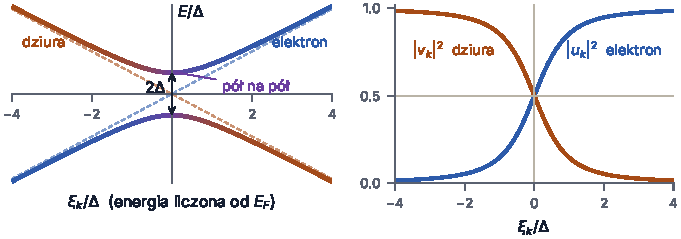
\includegraphics[width=0.8\linewidth]{fig/final/bogolubow.pdf}\\
  \podpis{daleko od $E_F$: zwykły elektron albo dziura; \ przy $E_F$: \textcolor{mPurple}{pół na pół} — i~przerwa $2\Delta$}
\end{frame}

% plan: relacja komutacji hamiltonianu z operatorem gamma → γ†(E) = γ(−E)
\begin{frame}{Symetria cząstka–dziura}
  \begin{columns}[c]
    \begin{column}{0.58\textwidth}
      $[H, \gamma_E^\dagger] = E\,\gamma_E^\dagger$
        \hfill \podpis{$\gamma_E^\dagger$ dodaje energię $E$}\\[3mm]
      sprzężenie hermitowskie:\\[1mm]
      $[H, \gamma_E] = -E\,\gamma_E$
        \hfill \podpis{$\gamma_E$ dodaje energię $-E$}\\[3mm]
      to samo równanie co dla $\gamma_{-E}^\dagger$:\\[2mm]
      \centering
      \duza{$\gamma^\dagger(E) = \gamma(-E)$}\\[1mm]
      \podpis{utworzyć kwazicząstkę o~energii $E$ = usunąć kwazicząstkę o~energii $-E$}
    \end{column}
    \begin{column}{0.38\textwidth}
      \centering
      \begin{tikzpicture}[y=0.74cm]
        \fill[mRed!9] (-0.2,-1) rectangle (2.6,1);
        \draw[-{Stealth}, mGray] (0,-3) -- (0,3.1) node[above, text=mDark] {$E$};
        \node[font=\scriptsize, text=mRed] at (0.7,-0.5) {przerwa};
        \foreach \e/\b in {1.3/30, 1.9/34, 2.6/38} {
          \draw[thick, mBlue] (0.4,\e) -- (1.0,\e);
          \draw[thick, mRed] (0.4,-\e) -- (1.0,-\e);
          \draw[{Stealth}-{Stealth}, mGray!70] (1.12,\e) to[bend left=\b] (1.12,-\e);
        }
        \node[font=\scriptsize, anchor=east] at (0.38,2.6) {$+E$};
        \node[font=\scriptsize, anchor=east] at (0.38,-2.6) {$-E$};
        \node[font=\large, text=mRed] at (0.7,0.2) {?};
        \draw (-0.08,1) -- (0.08,1) node[left=3pt, font=\scriptsize] {$\Delta$};
        \draw (-0.08,-1) -- (0.08,-1) node[left=3pt, font=\scriptsize] {$-\Delta$};
      \end{tikzpicture}\\
      \podpis{widmo symetryczne:\\ każdy stan liczony dwa razy}
    \end{column}
  \end{columns}
  \zrodlo{\LF, wz.~(43)–(47)}
\end{frame}

% plan: przejście do fermionów Majorany — E = 0; czego brakuje (spin, przerwa); styk
\begin{frame}{$E = 0$: Majorana — czego jeszcze brakuje?}
  \centering
  $\gamma^\dagger(E) = \gamma(-E)$ \quad ⇒ \quad dla $E = 0$: \quad
  \duza{$\gamma_0^\dagger = \gamma_0$}\\
  \podpis{stan nadprzewodnika przy zerowej energii \alert{jest} fermionem Majorany}\\[6mm]
  \raggedright
  \karta[mGreen]{12.6cm}{\tak\ \ superpozycja elektronu i~dziury — daje ją \alert{nadprzewodnik}}\\[2mm]
  \karta[mRed]{12.6cm}{\nie\ \ $E = 0$ — w~nadprzewodniku $|E| \ge \Delta$: w~przerwie nie ma stanów}\\[2mm]
  \karta[mRed]{12.6cm}{\nie\ \ spin: $\gamma^\dagger = u\,c^\dagger_\uparrow + v\,c_\downarrow \neq \gamma$ —
    elektron $\uparrow$ i~dziura $\downarrow$ to różne stany}
  \uwaga{Pomysł: szukać na \alert{styku} nadprzewodnika z~metalem / półprzewodnikiem
    (stany w~przerwie, odbicie Andriejewa) i~pozbyć się spinu → model Kitajewa.}
\end{frame}

% plan: najprostszy model — łańcuch Kitajewa; hamiltonian jak w artykule wz. (1)
\begin{frame}{Łańcuch Kitajewa (2001)}
  \centering
  \lancuch{0}\\[3mm]
  elektrony \alert{bez spinu} (jeden rodzaj) w~łańcuchu 1D\\
  parowanie \alert{sąsiadów} o~tym samym spinie (typ $p$)
  \[
    H = -\nb{\mu}\sum_{i=1}^{N} c_i^\dagger c_i
      \;-\; \sum_{i=1}^{N-1}\bigl(\textcolor{mGreen}{t}\,c_i^\dagger c_{i+1}
      + \cz{\Delta}\,c_{i+1}c_i + \hc\bigr)
  \]
  \podpis{\nb{$\mu$ — potencjał chemiczny} \quad · \quad \textcolor{mGreen}{$t$ — przeskok}
    \quad · \quad \cz{$\Delta$ — parowanie (przerwa)}}
  \uwaga{Znak przy $\Delta$ jak u~Kitajewa — wtedy niesparowane są $\gamma_{1,1}$ i~$\gamma_{N,2}$, jak na rys.~1 w~\LF.
    W~\LF\ wz.~(1) ma $\Delta\,c_ic_{i+1}$, z~czym nie wychodzi ich wz.~(6).}
  \zrodlo{A.\,Yu.~Kitaev, Phys.-Usp. 44, 131 (2001); \LF\ = M.~Leijnse, K.~Flensberg, Semicond. Sci. Technol. 27, 124003 (2012), wz.~(1)}
\end{frame}

% plan: zapisujemy równanie za pomocą operatorów Majorany
\begin{frame}{Zapis w~operatorach Majorany}
  \centering
  w~każdym węźle: \ $c_i = \tfrac12\,(\gamma_{i,1} + i\gamma_{i,2})$\\[2mm]
  \begin{align*}
    c_i^\dagger c_i &= \tfrac12\,\bigl(1 + i\gamma_{i,1}\gamma_{i,2}\bigr)\\
    c_i^\dagger c_{i+1} + \hc &= \tfrac{i}{2}\,\bigl(\gamma_{i,1}\gamma_{i+1,2} - \gamma_{i,2}\gamma_{i+1,1}\bigr)\\
    c_{i+1}c_i + \hc &= -\tfrac{i}{2}\,\bigl(\gamma_{i,1}\gamma_{i+1,2} + \gamma_{i,2}\gamma_{i+1,1}\bigr)
  \end{align*}
  ⇓
  \[
    H = -\frac{\mu}{2}\sum_{i}\bigl(1 + i\,\nb{\gamma_{i,1}\gamma_{i,2}}\bigr)
      + \frac{i}{2}\sum_{i}\Bigl[(t + \Delta)\,\cz{\gamma_{i,2}\gamma_{i+1,1}}
      + (\Delta - t)\,\textcolor{mGray}{\gamma_{i,1}\gamma_{i+1,2}}\Bigr]
  \]
  \podpis{\nb{w~węźle} \quad · \quad \cz{sąsiednie połówki} \quad · \quad \textcolor{mGray}{„na krzyż”}}
\end{frame}

% plan: specjalny punkt μ = 0, t = Δ; postać diagonalna, ale jeszcze niewidoczna
\begin{frame}{Punkt specjalny: $\mu = 0$, \ $t = \Delta$}
  \begin{columns}[c]
    \begin{column}{0.44\textwidth}
      \centering
      $\mu = 0$: znika człon \nb{w~węźle}\\
      $\Delta = t$: znika człon \textcolor{mGray}{„na krzyż”}\\[5mm]
      {\Large $\displaystyle H = i t\sum_{i=1}^{N-1}\gamma_{i,2}\,\gamma_{i+1,1}$}\\[4mm]
      zostają tylko \cz{sąsiednie połówki}\\[3mm]
      \podpis{to już postać diagonalna — tylko jeszcze tego nie widać}
    \end{column}
    \begin{column}{0.54\textwidth}
      \centering
      \obrazek{0.93\linewidth}{fig/ref/rys1.png}
    \end{column}
  \end{columns}
  \zrodlo{Rys.: \LF, rys.~1 (w~podpisie artykułu indeksy końcowych Majoran są zamienione)}
\end{frame}

% plan: nowy operator jako parowanie przesuniętych Majoran; H = ε n̂; energia 2t
\begin{frame}{Nowe fermiony z~przesuniętych połówek}
  \centering
  \lancuch{1}\\[3mm]
  \begin{columns}[c]
    \begin{column}{0.6\textwidth}
      \centering
      $\tilde c_i = \tfrac12\bigl(\gamma_{i,2} + i\gamma_{i+1,1}\bigr)$
      \ ⇒ \ $i\gamma_{i,2}\gamma_{i+1,1} = 2\tilde c_i^\dagger\tilde c_i - 1$\\[4mm]
      {\Large $\displaystyle H = 2t\sum_{i=1}^{N-1}\tilde c_i^\dagger\tilde c_i + \text{const}$}\\[1mm]
      \podpis{postać diagonalna: \ $H = \sum \varepsilon\,\hat n$}
    \end{column}
    \begin{column}{0.36\textwidth}
      \centering
      \duza{$2t$}\\
      \podpis{koszt każdego wzbudzenia\\ = przerwa łańcucha ($= 2\Delta$)}
    \end{column}
  \end{columns}
\end{frame}

% plan: para na końcach znika z hamiltonianu — zero energii; operator kreacji dla połówek
\begin{frame}{Na końcach zostaje para bez energii}
  \centering
  \lancuch{2}\\[1mm]
  \karta[koral]{3.75cm}{\footnotesize $\gamma_{1,1}$, $\gamma_{N,2}$ — \alert{nie ma ich w~$H$}:\\
    $[H, \gamma_{1,1}] = [H, \gamma_{N,2}] = 0$\\ ⇒ energia \alert{zero}}\hfill
  \karta[mRed]{3.75cm}{\footnotesize $2N$ Majoran = $N-1$ fermionów $\tilde c_i$ + 2~samotne końce\\
    → jeden fermion \alert{nielokalny} $\tilde c_M$}\hfill
  \karta[mBlue]{3.75cm}{\footnotesize stan podstawowy: $\ket{0}$ i~$\tilde c_M^\dagger\ket{0}$\\
    parzysta / nieparzysta liczba elektronów — \alert{ta sama} energia}
  \zrodlo{\LF, wz.~(9)}
\end{frame}

% plan: (uzupełnienie) poza punktem specjalnym — faza topologiczna, własna symulacja
\begin{frame}{Poza punktem specjalnym}
  \centering
  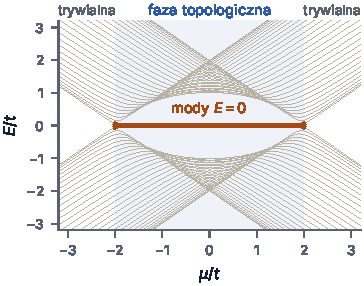
\includegraphics[height=4.15cm]{fig/final/kitaev_widmo.pdf}\hfill
  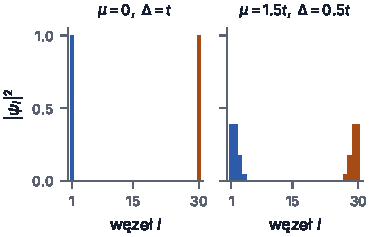
\includegraphics[height=4.15cm]{fig/final/kitaev_mody.pdf}\\[3mm]
  mody $E = 0$ przeżywają dla $|\mu| < 2t$ — \alert{faza topologiczna};\
  poza punktem specjalnym zanikają $\sim e^{-x/\xi}$ od końców
  \zrodlo{Obliczenia własne (\texttt{sim/wykresy.py}): widmo BdG łańcucha $N{=}30$, $\Delta{=}0.5\,t$}
\end{frame}

% =============================================================================
\czesc{4}{Właściwości Majoran}{zawsze parami, $\gamma^2 = 1$,\\pomiar i~statystyka nieabelowa}
% =============================================================================

% plan: zawsze parzysta liczba — n fermionów tworzy 2n Majoran
\begin{frame}{Zawsze parami}
  \begin{columns}[c]
    \begin{column}{0.5\textwidth}
      \centering
      {\tytulowa\Large $n$ fermionów \ $\leftrightarrow$ \ $2n$ Majoran}\\[7mm]
      \begin{tikzpicture}
        \foreach \y/\a/\b in {0/1/2, -1.3/3/4} {
          \fill[mDark!12, rounded corners=2pt] (0,\y-0.12) rectangle (4.2,\y+0.12);
          \fill[koral] (0.18,\y) circle (0.1);
          \fill[koral] (4.02,\y) circle (0.1);
          \node[font=\scriptsize, above=1.5mm] at (0.18,\y) {$\gamma_\a$};
          \node[font=\scriptsize, above=1.5mm] at (4.02,\y) {$\gamma_\b$};
          \draw[koral!70, dashed] (0.18,\y-0.15) .. controls (1.2,\y-0.6) and (3,\y-0.6) .. (4.02,\y-0.15);
        }
      \end{tikzpicture}\\[2mm]
      \podpis{4 Majorany = 2 fermiony = $2^2$ stany}
    \end{column}
    \begin{column}{0.46\textwidth}
      \begin{itemize}\setlength{\itemsep}{3mm}
        \item Majorany powstają \alert{parami} — łańcuch ma dwa końce
        \item sama Majorana \alert{nie niesie} stanu — stan ma dopiero para
        \item liczba Majoran jest zawsze \alert{parzysta}
      \end{itemize}
    \end{column}
  \end{columns}
  \uwaga{$2n$ Majoran → $2^n$ stanów: na jedną Majoranę przypada „$\sqrt2$ stanu”.}
\end{frame}

% plan: nie działa zakaz Pauliego — {γi,γj} = 2δij ⇒ γ² = 1
\begin{frame}{$\gamma^2 = 1$: zakaz Pauliego nie działa}
  \begin{columns}[T]
    \begin{column}{0.46\textwidth}
      \centering
      \textbf{fermion}\\[3mm]
      $\{c_i^\dagger, c_j^\dagger\} = 0$\\[2mm]
      ⇓\\[2mm]
      \duza{$(c^\dagger)^2 = 0$}\\[2mm]
      \podpis{drugi raz obsadzić się \alert{nie da}}
    \end{column}
    \begin{column}{0.46\textwidth}
      \centering
      \textbf{Majorana}\\[3mm]
      $\{\gamma_i, \gamma_j\} = 2\delta_{ij}$\\[2mm]
      ⇓\\[2mm]
      \duza{$\gamma^2 = 1$}\\[2mm]
      \podpis{„obsadzamy” drugi raz — i~wracamy do punktu wyjścia}
    \end{column}
  \end{columns}
  \vspace{8mm}
  \centering
  $\gamma\gamma\ket{\psi} = \ket{\psi}$ \quad — \quad stan „obsadzony dwa razy” to ten sam stan
\end{frame}

% plan: nie ma sensu pytać o obsadzenie — γ†γ = 1 zawsze
\begin{frame}{Ile jest Majoran w~stanie? Pytanie bez sensu}
  \centering
  próba: \quad $\hat n_\gamma = \gamma^\dagger\gamma = \gamma^2 = $ \duza{$1$}\\
  \podpis{\alert{zawsze} $1$ — w~każdym stanie, więc nic nie mierzy}\\[8mm]
  \karta[mBlue]{5.4cm}{obsadzenie ma dopiero \alert{para}:\\[1mm]
    $\hat n = \tilde c^\dagger\tilde c = \tfrac12\,(1 + i\gamma_1\gamma_2)$}\qquad
  \karta[mRed]{5.4cm}{parzystość pary:\\[1mm]
    $P = -i\gamma_1\gamma_2 = 1 - 2\hat n = \pm1$}
\end{frame}

% plan: pomiar pojedynczej Majorany nie ma sensu
\begin{frame}{Pomiar pojedynczej Majorany nie ma sensu}
  \centering
  \begin{tikzpicture}
    \fill[mPurple!25] (0,0.5) rectangle (8,0.72);
    \fill[mDark!18, rounded corners=3pt] (0,0) rectangle (8,0.5);
    \node[font=\tiny, text=mPurple] at (4,0.61) {nadprzewodnik};
    \node[font=\scriptsize] at (4,0.25) {nanodrut};
    \fill[koral] (0.35,0.25) circle (0.13);
    \fill[koral] (7.65,0.25) circle (0.13);
    \node[below=1pt] at (0.35,0) {$\gamma_1$};
    \node[below=1pt] at (7.65,0) {$\gamma_2$};
    \draw[dashed, thick, mBlue] (0.35,0.75) .. controls (2,1.9) and (6,1.9) .. (7.65,0.75);
    \node[mBlue, fill=kartabg, draw=linia!70, rounded corners=1.6pt, inner sep=2.5pt] at (4,1.62) {$\tilde c = \tfrac12(\gamma_1 + i\gamma_2)$};
    \draw[-{Stealth}, very thick, mRed, decorate,
          decoration={zigzag, segment length=4pt, amplitude=1.5pt, post length=3pt}]
          (-1.3,1.3) -- (0.15,0.45);
    \node[font=\scriptsize] at (-1.5,1.6) {lokalny szum};
    \draw[{Stealth}-{Stealth}, mGray] (0.35,-0.65) -- node[below, font=\scriptsize] {$L \gg \xi$} (7.65,-0.65);
  \end{tikzpicture}\\[7mm]
  \karta[mRed]{3.75cm}{\footnotesize $\gamma = c + c^\dagger$ zmienia liczbę elektronów o~1 — \alert{nie} jest obserwablą}\hfill
  \karta[mBlue]{3.75cm}{\footnotesize mierzalna jest tylko parzystość pary $-i\gamma_1\gamma_2$ — \alert{oba końce} naraz}\hfill
  \karta[mGreen]{3.75cm}{\footnotesize szum widzi \alert{pół} fermionu: informacja zapisana nielokalnie, błędy $\propto e^{-L/\xi}$}
\end{frame}

% plan: statystyka nieabelowa
\begin{frame}{Statystyka nieabelowa}
  \begin{columns}[c]
    \begin{column}{0.34\textwidth}
      \centering
      \begin{tikzpicture}[scale=0.9]
        \draw[-{Stealth}, mGray] (-0.7,0) -- (-0.7,3.2) node[above, font=\small, text=mDark] {czas};
        \draw[very thick, koral] (0,0) -- (0,3);
        \draw[very thick, koral] (3,0) -- (3,3);
        \begin{scope}[even odd rule]
          \clip (-1,-0.5) rectangle (4,3.5) (1.5,1.5) circle (0.2);
          \draw[very thick, mGreen] (2,0) -- (2,1) .. controls (2,1.5) and (1,1.5) .. (1,2) -- (1,3);
        \end{scope}
        \draw[very thick, mBlue] (1,0) -- (1,1) .. controls (1,1.5) and (2,1.5) .. (2,2) -- (2,3);
        \foreach \x/\l in {0/1, 1/2, 2/3, 3/4} \node[below, font=\small] at (\x,0) {$\gamma_\l$};
      \end{tikzpicture}
    \end{column}
    \begin{column}{0.62\textwidth}
      fermiony: zamiana → liczba $-1$\\[2mm]
      Majorany: zamiana → \alert{operator}
      \[ U_{ij} = e^{\frac{\pi}{4}\gamma_i\gamma_j} = \tfrac{1}{\sqrt2}\,(1 + \gamma_i\gamma_j) \]
      \[ U_{12}\,U_{23} \neq U_{23}\,U_{12} \quad \text{— \alert{kolejność ma znaczenie}} \]
      wynik zależy od tego, \emph{jak} splotły się ścieżki (braiding)\\[2mm]
      \podpis{→ pomysł na topologiczny komputer kwantowy: 4 Majorany = 1 kubit}
    \end{column}
  \end{columns}
  \zrodlo{D.\,A.~Ivanov, Phys. Rev. Lett. 86, 268 (2001); \LF, rozdz.~3}
\end{frame}

% podsumowanie właściwości
\begin{frame}{Fermion a~Majorana}
  \centering
  \renewcommand{\arraystretch}{1.75}
  \begin{tabular}{lcc}
    & fermion $c$ & Majorana $\gamma$\\
    \midrule
    sprzężenie    & $c^\dagger \neq c$                  & $\cz{\gamma^\dagger = \gamma}$\\
    kwadrat       & $c^2 = 0$                           & $\cz{\gamma^2 = 1}$\\
    antykomutator & $\{c_i, c_j^\dagger\} = \delta_{ij}$ & $\{\gamma_i, \gamma_j\} = 2\delta_{ij}$\\
    obsadzenie    & $c^\dagger c \in \{0, 1\}$          & $\cz{\gamma^\dagger\gamma = 1}$ — zawsze\\
    wymiana       & $-1$                                & \cz{macierz} (nieabelowa)\\
    energia       & dowolna                             & $\cz{E = 0}$\\
  \end{tabular}
\end{frame}

% most do części 5
\begin{frame}{Podsumowanie: droga do Majorany}
  \centering\vfill
  \begin{tikzpicture}[
      k/.style={fill=kartabg, draw=linia!70, line width=0.3pt, rounded corners=1.6pt,
                align=center, font=\small\bezdzielenia, text=mDark, minimum height=1.25cm,
                text width=2.75cm},
      s/.style={-{Stealth}, thick, mGray}]
    \node[k] (a) at (0,0)      {cząstka /\\ antycząstka (Dirac)};
    \node[k] (b) at (3.45,0)    {$c$, $c^\dagger$\\ antykomutacja};
    \node[k] (c) at (6.9,0)      {$\gamma = \gamma^\dagger$\\ pół fermionu};
    \node[k] (d) at (10.35,0)   {nadprzewodnik:\\ $e + h$, \ $E = 0$?};
    \node[k] (e) at (10.35,-2.3) {łańcuch Kitajewa:\\ Majorany na końcach};
    \node[k] (f) at (6.9,-2.3)   {$\gamma^2 = 1$,\\ nieabelowe};
    \node[k, draw=mRed, fill=mRed!7, line width=0.9pt] (g) at (3.45,-2.3)
      {nanodrut,\\ nadprzewodnik,\\ pole $B$};
    \draw[s] (a) -- (b);
    \draw[s] (b) -- (c);
    \draw[s] (c) -- (d);
    \draw[s] (d) -- (e);
    \draw[s] (e) -- (f);
    \draw[s] (f) -- (g);
    \node[font=\small, text=mRed, anchor=east] at ([xshift=-5mm]g.west) {część 5 →};
  \end{tikzpicture}
  \vfill
\end{frame}

% =============================================================================
\section{Realizacja fizyczna}
% =============================================================================
\ifnum\wersjafinalna=1\relax
  % --- część 5: slajdy kolegi (31 stron, 16:9, skalowane na całą stronę) ----
  % jasna strona kolegi: numer w prawym dolnym rogu jak na naszych slajdach
  \newcommand{\slajdKolegi}[1]{%
    {\setbeamertemplate{background canvas}{%
       \includegraphics[page=#1, width=\paperwidth, height=\paperheight]{\plikKolegi}}%
     \begin{frame}\mbox{}\end{frame}}}
  % granatowa strona kolegi: bez numeru; #2 = dodatkowa nakładka TikZ
  \newcommand{\slajdKolegiCiemny}[2]{%
    {\setbeamertemplate{background canvas}{%
       \includegraphics[page=#1, width=\paperwidth, height=\paperheight]{\plikKolegi}}%
     \begin{frame}[plain]#2\end{frame}}}

  % strona tytułowa kolegi = otwarcie części 5: dopisujemy „Część 5”
  % i zasłaniamy pole „[Imiona i nazwiska] · [data]”
  \slajdKolegiCiemny{1}{%
    \begin{naStronie}
      \node[anchor=base west, inner sep=0, font=\small, text=jasny]
        at (10.8mm,{-(24.5mm)}) {Część 5 \ \textperiodcentered\ \ Realizacja fizyczna};
      \fill[mDark] (10mm,{-(57.6mm)}) rectangle (48mm,{-(63.4mm)});
      \ifdefempty{\prelegentB}{}{%
        \node[anchor=base west, inner sep=0, font=\fontsize{7}{8}\selectfont, text=jasny]
          at (10.8mm,{-(61.3mm)}) {\prelegentB};}
    \end{naStronie}}
  \slajdKolegi{2}
  \slajdKolegi{3}
  \slajdKolegi{4}
  \slajdKolegi{5}
  \slajdKolegi{6}
  \slajdKolegi{7}
  \slajdKolegi{8}
  \slajdKolegi{9}
  \slajdKolegi{10}
  \slajdKolegi{11}
  \slajdKolegi{12}
  \slajdKolegi{13}
  \slajdKolegi{14}
  \slajdKolegi{15}
  \slajdKolegi{16}
  \slajdKolegi{17}
  \slajdKolegiCiemny{18}{}
  \slajdKolegi{19}
  \slajdKolegi{20}
  \slajdKolegi{21}
  \slajdKolegi{22}
  \slajdKolegi{23}
  \slajdKolegi{24}
  \slajdKolegi{25}
  \slajdKolegi{26}
  \slajdKolegi{27}
  \slajdKolegi{28}
  \slajdKolegi{29}
  \slajdKolegi{30}
  \slajdKolegiCiemny{31}{}
\else
  {\ciemne
  \begin{frame}[plain]
    \begin{naStronie}
      \node[anchor=base west, inner sep=0, font=\small, text=jasny]
        at (10.8mm,{-(24.5mm)}) {Część 5};
      \node[anchor=north west, inner sep=0, text=tlo, text width=78mm, align=left,
            font=\tytulowa\fontsize{28}{29}\selectfont] at (10.8mm,{-(28.6mm)})
            {Realizacja fizyczna};
      \node[anchor=north west, inner sep=0, text=jasny, font=\fontsize{8.6}{11}\selectfont]
        at (10.8mm,{-(43mm)}) {slajdy kolegi — pełna wersja: \texttt{prezentacja\_finalna.pdf}};
      \mapaPionowa{5}
    \end{naStronie}
  \end{frame}}
\fi

% =============================================================================
\section*{Bibliografia}
\begin{frame}{Bibliografia}
  \fontsize{7.8}{9.6}\selectfont
  \begin{itemize}\setlength{\itemsep}{1.2mm}
    \item[{[1]}] M.~Leijnse, K.~Flensberg, \emph{Introduction to topological superconductivity
          and Majorana fermions}, Semicond. Sci. Technol. \textbf{27}, 124003 (2012), arXiv:1206.1736 — \LF
    \item[{[2]}] V.~Mourik i~in., \emph{Signatures of Majorana fermions in hybrid superconductor–semiconductor
          nanowire devices}, Science \textbf{336}, 1003 (2012) — część~5
    \item[{[3]}] \emph{Second quantization: basics}, Dr Mitchell's physics channel (YouTube),
          \url{https://youtu.be/6RhjrdnDUNI}
    \item[{[4]}] S.~Frolov, \emph{Majorana Fermions in Nanowires} (YouTube),
          \url{https://youtu.be/kh1u9Q5D47w}
    \item[{[5]}] 3Blue1Brown, \emph{But what is quantum computing? (Grover's Algorithm)} (YouTube),
          \url{https://youtu.be/RQWpF2Gb-gU}
    \item[{[6]}] Claude (Anthropic), \url{https://claude.ai}
  \end{itemize}
  \vspace{2mm}
  {\fontsize{6.6}{8.2}\selectfont\color{mGray}
  Cytowane na slajdach:
  P.\,A.\,M.~Dirac, Proc. R. Soc. Lond. A \textbf{117}, 610 (1928) \textperiodcentered{}
  E.~Majorana, Nuovo Cimento \textbf{14}, 171 (1937) \textperiodcentered{}
  C.\,D.~Anderson, Phys. Rev. \textbf{43}, 491 (1933) \textperiodcentered{}
  H.~Kamerlingh Onnes, Commun. Phys. Lab. Leiden \textbf{120b} (1911) \textperiodcentered{}
  W.~Meissner, R.~Ochsenfeld, Naturwissenschaften \textbf{21}, 787 (1933) \textperiodcentered{}
  L.\,N.~Cooper, Phys. Rev. \textbf{104}, 1189 (1956) \textperiodcentered{}
  J.~Bardeen, L.\,N.~Cooper, J.\,R.~Schrieffer, Phys. Rev. \textbf{108}, 1175 (1957) \textperiodcentered{}
  N.\,N.~Bogoliubov, Nuovo Cimento \textbf{7}, 794 (1958) \textperiodcentered{}
  I.~Giaever, Phys. Rev. Lett. \textbf{5}, 147 (1960) \textperiodcentered{}
  A.\,F.~Andreev, Sov. Phys. JETP \textbf{19}, 1228 (1964) \textperiodcentered{}
  A.\,Yu.~Kitaev, Phys.-Usp. \textbf{44}, 131 (2001) \textperiodcentered{}
  D.\,A.~Ivanov, Phys. Rev. Lett. \textbf{86}, 268 (2001) \textperiodcentered{}
  Ch.~Kittel, \emph{Introduction to Solid State Physics}, Wiley \textperiodcentered{}
  N.\,W.~Ashcroft, N.\,D.~Mermin, \emph{Solid State Physics}, Saunders.\par}
\end{frame}

\end{document}
